% !TeX spellcheck = en_GB
\documentclass{beamer}\mode<presentation>{\usetheme{AMSCesenaPurpleAndGold}}
\setbeamertemplate{bibliography item}{\insertbiblabel}

\usepackage{common}

\newcommand{\labN}{1}

\title[L\labN{} -- Build Automation 101]{L\labN{} -- Build Automation 101}
%
\subtitle[SD]{Distributed Systems / Technologies}
%
\author[Ciatto \and Omicini]
{\emph{Giovanni Ciatto} \and Andrea Omicini\\
\texttt{giovanni.ciatto@unibo.it \and andrea.omicini@unibo.it}}
%
\institute[DISI, Univ. Bologna]
{Dipartimento di Informatica -- Scienza e Ingegneria (DISI)\\\textsc{Alma Mater Studiorum} -- Universit{\`a} di Bologna a Cesena}
%
\date[A.Y. 2020/2021]{Academic Year 2020/2021}

\setbeamercovered{transparent}

\AtBeginSection[]
{
\begin{frame}[c]\frametitle{Next in Line\ldots}
%    \begin{multicols}{2}
        \tableofcontents[sectionstyle=show/shaded, subsectionstyle=show/hide, subsubsectionstyle=hide/hide]
%    \end{multicols}
\end{frame}
}

\begin{document}

\maketitle

\begin{frame}[c]\frametitle{Outline}
    % \begin{multicols}{2}
	    \tableofcontents[sectionstyle=show/show, subsectionstyle=show/show, subsubsectionstyle=show/show]
    % \end{multicols}
\end{frame}

\section{Motivation}

\begin{frame}[allowframebreaks]
\frametitle{Motivation}

    \begin{itemize}
        \item Real world (distributed) applications are made up of several \alert{components} which need to be \alert{deployed} on one or more machines
        %
        \begin{itemize}
            \item possibly in an orderly fashion
        \end{itemize}

        \bigskip

        \item Furthermore, only rarely people write software \alert{from scratch}
        %
        \begin{itemize}
            \item more commonly, software \alert{depends} from other software
            %
            \begin{itemize}
                \item which may depend on further software, and so on
            \end{itemize}

            \item[$\rightarrow$] dependencies cannot be \alert{manually} handled
            %
            \begin{itemize}
                \item error prone, time consuming task
            \end{itemize}
        \end{itemize}

        \framebreak

        \item In projects/exercises, you may need to write, compile, \alert{deploy}, \& start several processes in a given \alert{order}, possibly multiple \alert{times}
        %
        \begin{itemize}
            \item furthermore we may will to exploit \alert{open-source libraries} from the Internet
        \end{itemize}

        \bigskip


        \item We will extensively leverage \alert{Build Automation} in our activities to automate most low level operations
        %
        \begin{itemize}
            \item in an IDE-independent way
            \item (activities include exercises and final projects :)
        \end{itemize}

    \end{itemize}

\end{frame}

% \begin{frame}
% \frametitle{Lecture goals II}

%     \begin{itemize}
%         \item<1> In this course, you may need a way to reproduce Lab exercises on your personal computers, possibly simulating a distributed environment

%         \vfill{}

%         \item<2> Furthermore, you must be able to submit your homeworks/projects being sure they will run on other computer too
%         \begin{itemize}
%             \item<2> Avoiding the situation \emph{``No, I swear, it used to work on my PC''} :)

%             \item<2>[!] Making your results more durable and \alert{reproducible}
%         \end{itemize}

%         \vfill{}

%         \item<3>[$\rightarrow$] You will learn some fundamentals of:
%         \begin{itemize}
%             \item<3> Build \& automation systems (e.g. \href{https://gradle.org/}{Gradle})
%             \item<3> Container Engines (e.g. \href{https://www.docker.com/}{Docker})
%         \end{itemize}

%         \vfill{}

%         \item<4> Because of Lab-0, you are assumed to:
%         \begin{itemize}
%             \item<4> have properly installed Gradle and Docker on your personal PC
%             \item<4> have a Docker ID with your \texttt{@studio.unibo.it} email address
%         \end{itemize}
%     \end{itemize}

% \end{frame}

\section{Build Automation Systems}

\subsection{Overview}

\begin{frame}{Build Automation Systems}
    Build automation systems \alert{automate} several sub-tasks of the SW developing \& engineering process, like for instance:
    %
    \begin{multicols}{2}
        \begin{itemize}
            \item Dependencies management

            \item \alert{Compilation}

            \item Code generation

            \item Testing

            \item Execution

            \item Artefact generation
            %
            \begin{itemize}
                \item[eg] \texttt{.jar} files
            \end{itemize}

            \item Release publication/upload
        \end{itemize}
    \end{multicols}
    %
    just to cite some.

    \vfill

    \begin{itemize}

        \item Remember the time spent configuring someone else's Eclipse project?
        %
        \begin{itemize}
            \item we are targeting that problem
        \end{itemize}

        \item[!] Plus, build automation systems are very handy when combined with Containers, e.g. for Continuous Integration

    \end{itemize}


\end{frame}

\subsection{Gradle}

\begin{frame}{Why Build Automation Systems}
    We will leverage \alert{Gradle} as a build automation system for JVM-based application in order to automate your exercises/projects:
    %
    \begin{itemize}
        \item dependencies management
        \item compilation
        \item launch by command line
    \end{itemize}

    \vfill

    (Of course, alternatives exist for other platforms)

    \vfill

    \begin{block}{From now on}
        \begin{itemize}
            \item JVM projects \emph{should} be submitted as self-contained Gradle projects
        \end{itemize}
    \end{block}
\end{frame}

\begin{frame}
\frametitle{Gradle I}

    Gradle is our build automation of choice
    %
    \vfill
    %
    \begin{itemize}
        \item It assumes each project to adhere to a well defined \alert{directory structure}

        \vfill

        \item A \alert{\texttt{gradlew}} (or \texttt{gradlew.bat}, on Windows systems) script is assumed to be present within the project root directory
        %
        \begin{itemize}
        	\item it is called the \alert{Gradle wrapper}
        	\item the directory containing it is called the \alert{root of the project}
        \end{itemize}

        \vfill

        \item Dependencies are just \alert{declared} into a \alert{\texttt{build.gradle(.kts)}} file, along with their versions
        %
        \begin{itemize}
            \item no \texttt{.jar} file must/should be provided, in the general case
        \end{itemize}
    \end{itemize}

\end{frame}

\begin{frame}
\frametitle{Gradle II}
    \begin{itemize}
        \item Under such hypotheses, developers can execute several tasks on the project by calling the \texttt{gradlew} script as follows:
        \begin{itemize}
            \item[\$] \texttt{\alert{./}gradlew \alert{<task>}} \quad (on Unix)
            \item[] or
            \item[$>$] \texttt{\alert{.$\backslash$}gradlew \alert{<task>}} \quad (on Windows)
        \end{itemize}

        \vfill

        \item If Gradle is properly installed on your system, you don't need the \texttt{gradlew} script:
        \begin{itemize}
            \item[\$] \texttt{gradle \alert{<task>}} \quad (on both Unix and Windows)
        \end{itemize}

    \end{itemize}

\end{frame}

\begin{frame}
    \frametitle{Gradle III}
    \begin{itemize}

        \item The set of available tasks (for JVM apps) includes:
        %
        \begin{description}
            \item[\texttt{assemble}] | compiles the projects
            \item[\texttt{check}] | runs the user-defined tests
            \item[\texttt{build}] | runs the tests and (if no one fails) compiles the projects
            \item[\texttt{run}] | runs the application
            \item[\texttt{tasks}] | shows a list of available tasks
        \end{description}

        \vfill

        \item Dependencies between are as follows:
        %
        \begin{itemize}
            \item \texttt{run} $\rightarrow$ \texttt{build} $\rightarrow$ \texttt{check} $\rightarrow$ \texttt{assemble}

            \item so if you try to run an unassembled application, it will be
            %
            \begin{itemize}
                \item firstly \alert{assembled} (i.e., compiled)
                \item then \alert{checked} (i.e., tested)
                \item and finally \alert{run}
            \end{itemize}
        \end{itemize}
    \end{itemize}

\end{frame}

\subsubsection{Canonical Directory Structure}

\begin{frame}[fragile]
\frametitle{Canonical Directory Structure}

    % \lstinputlisting[language=]{./res/src/dir_structure}

\begin{Verbatim}[commandchars=\\\{\}]
\textcolor{blue}{my-project/}\dhint{The project root directory, named after it}
├── \textcolor{green}{gradlew}\dhint{The \emph{Gradle Wrapper} script, for Unix}
├── \textcolor{green}{gradlew.bat}\dhint{The \emph{Gradle Wrapper} script, for Windows}
├── \textcolor{olive}{build.gradle[.kts]}\dhint{The project setting \& tasks, in Gradle lang}
├─┬ \textcolor{cyan}{src/}\dhint{The \emph{source} folder: contains the project code}
│ ├─┬ main/\dhint{The 'main' \emph{source set}, contains the application code}
│ │ └─┬── java/\dhint{Java source files}
│ │   ├?─ kotlin/\dhint{Kotlin source files}
│ │   └?─ \textcolor{orange}{resources/}\dhint{The application resource files}
│ └?┬ test/\dhint{The 'test' \emph{source set}, contains the tests code}
│   └─┬?─ <other lang>/
│     └?─ \textcolor{orange}{resources/}
├?─ \textcolor{olive}{settings.gradle[.kts]}\dhint{Some minor project settings, in Gradle lang}
├?─ \textcolor{yellow}{gradle.properties}\dhint{A \href{https://en.wikipedia.org/wiki/.properties}{\emph{.properties} file} for default properties}
├── \textcolor{red}{gradle/}\dhint{Contains libraries for the Gradle Wrapper}
└── \textcolor{red}{build/}\dhint{Where compiled \emph{.class} and \emph{.jar} files are put}
\end{Verbatim}

\end{frame}

\subsubsection{Gradle Tasks \& Dependencies}

\begin{frame}[allowframebreaks]
\frametitle{Gradle Tasks \& Dependencies -- Try by Yourself}

    \columsHH{
        \begin{enumerate}
            \item Choose a project name
            %
            \begin{itemize}
                \item[eg] \alert{\texttt{my-app}}
            \end{itemize}
        
        	\medskip

            \item Create a directory named after the project and move your shell into it
            %
            \begin{itemize}
                \item[\$] \texttt{mkdir \alert{my-app}}
                \item[\$] \texttt{cd my-app}
                \item[\$] \texttt{gradle init --type java-application}
                \item[]
                \item[] (Works on both Unix and Windows)
            \end{itemize}
        
        	\medskip

            \item The directory structure shown on the right should have been created
        \end{enumerate}
    }{
        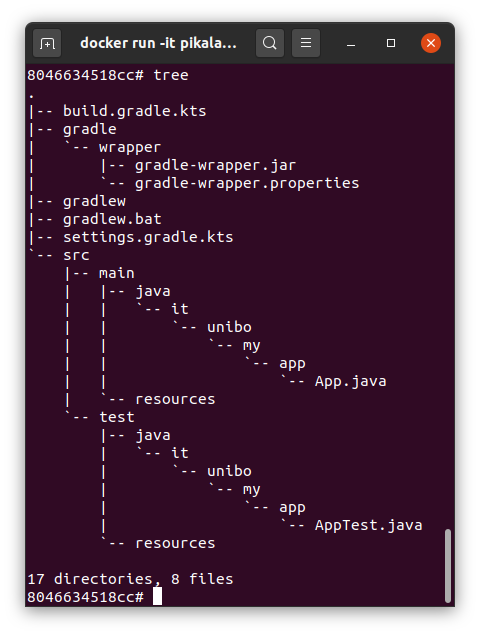
\includegraphics[width=\linewidth]{res/img/gradle_tree.png}
    }

    \framebreak

    \begin{enumerate}\setcounter{enumi}{3}
        \item Prefer \alert{Kotlin} as a build script DSL, and \alert{JUnit} as test framework

		\medskip
		
        \item Inspect the generated files structure \& look for the \texttt{App.java} file

		\medskip
	
        \item Run the application by typing:
        \begin{itemize}
            \item[\$] \texttt{./gradlew run}
            \item[] on Unix, or, in case of Windows:
            \item[$>$] \texttt{.$\backslash$gradlew run}
            \item[]
        \end{itemize}
    	
    	\medskip
    
        \item Re-run the application by typing:
        \begin{itemize}
            \item[\$] \texttt{./gradlew \alert{--no-daemon --console=plain} run}
            \item[] on Unix, or, in case of Windows:
            \item[$>$] \texttt{.$\backslash$gradlew \alert{--no-daemon --console=plain} run}
        \end{itemize}

        \medskip

        \item Can you spot the differences?
    \end{enumerate}

    \framebreak

    \begin{enumerate}\setcounter{enumi}{8}
        \item Now look at the \texttt{\alert{build.gradle.kts}} file
        \begin{itemize}
            \item depending on your specific Gradle version this may change slightly
        \end{itemize}
    \end{enumerate}
    %
    \lstinputlisting[language=Java]{./res/src/build.gradle.kts}

\end{frame}

\begin{frame}[c,allowframebreaks]{About Dependencies}

    Dependencies -- i.e., specific versions of artefacts -- can be added by appending to the \texttt{dependencies} section lines of the form
    %
    \begin{center}
        \texttt{implementation "<gropuId>}\alert{:}\texttt{<artifactId>}\alert{:}\texttt{<version>"}
    \end{center}
    %
    \begin{description}
        \item[\texttt{gropuId}] identifies a group of related artefacts
        \item[\texttt{artifactId}] identifies a specific artefact within the group
        \item[\texttt{version}] identifies a specific version of that artefact
    \end{description}

    \medskip

    BTW, versions are usually expressed through Semantic Versioning \ccite{semVer}
    %
    \begin{center}
        \texttt{"<MAJOR>}\alert{.}\texttt{<MINOR>}\alert{:}\texttt{<PATCH>"}
    \end{center}
    %
    \begin{description}
        \item[\texttt{MAJOR}] increases when non-retro-compatible changes are done
        \item[\texttt{MINOR}] increases when retro-compatible changes are done
        \item[\texttt{PATCH}] increases when implementation details are changed
    \end{description}

    \framebreak

    Artefacts -- along with their \texttt{groupId}, \texttt{artifactID} and \texttt{version} -- are hosted on repositories such as \href{https://search.maven.org/}{Maven Central} or \href{https://bintray.com/bintray/jcenter}{JCenter}
    %
    \begin{center}
        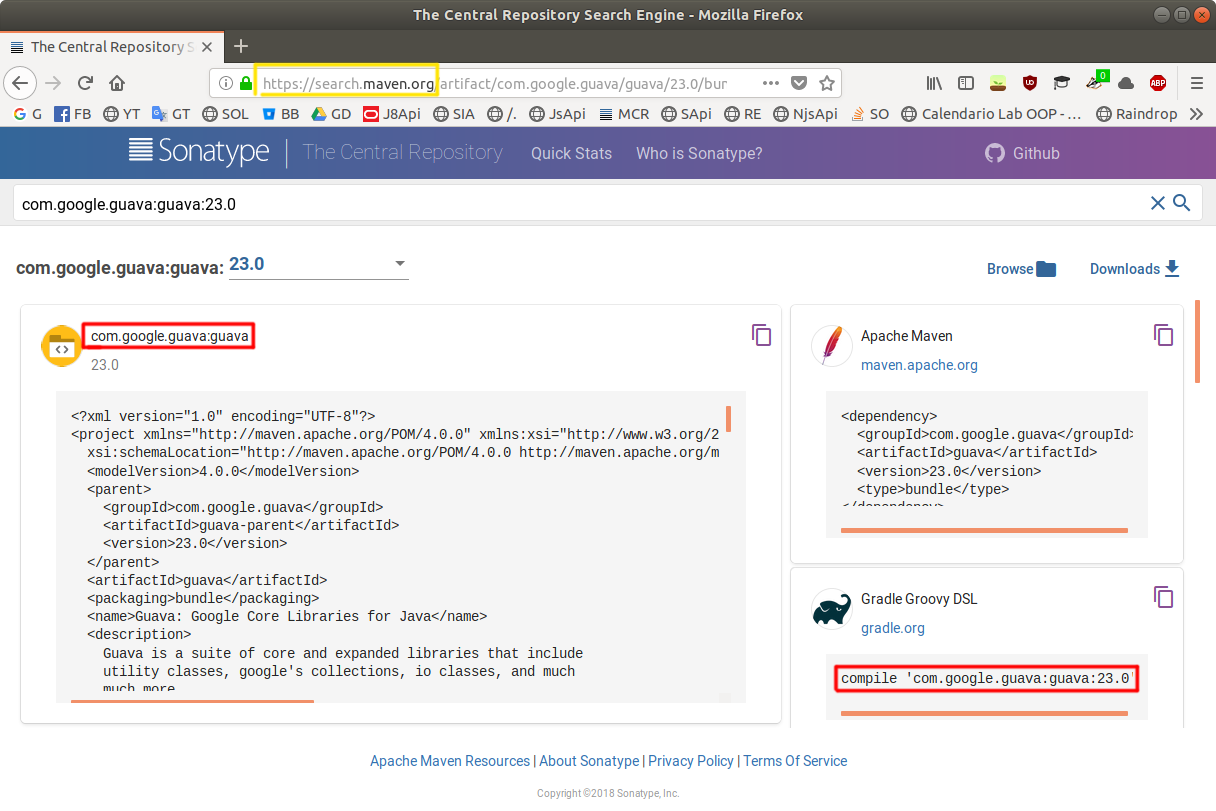
\includegraphics[width=.6\linewidth]{./res/img/mcr.png}

        {\scriptsize\url{https://search.maven.org/artifact/com.google.guava/guava/29.0-jre/bundle}}
    \end{center}

\end{frame}

\subsubsection{Gradle Properties}

\begin{frame}[allowframebreaks]
\frametitle{Gradle Properties -- Try it your self}
    \begin{enumerate}

        \item Try editing the \texttt{App.java} program in such a way it accepts some arguments, like for instance:
        %
        \lstinputlisting[language=Java]{./res/src/App.java}

        \item Try running it with
        \begin{itemize}
            \item[\$] \texttt{./gradlew run}
            \item[] or
            \item[$>$] \texttt{.$\backslash$gradlew run}
            \item[]
            \item do you expect this to work?
        \end{itemize}
    \end{enumerate}
    %
    \begin{itemize}
        \item[!] How to pass arguments to a Gradle task?
    \end{itemize}

    \framebreak

    \begin{enumerate}\setcounter{enumi}{2}
        \item Let's redefine the \texttt{run} task by \alert{adding} the following section to the \texttt{build.gradle.kts} file: \hint{help for backticks \href{https://stefanonegro.it/2013/04/15/backtick-e-tilde-con-una-tastiera-italiana}{here}}
        %
        \lstinputlisting[language=Java]{./res/src/run.task.kts}

        \item Try running it again, with:
        \begin{itemize}
            \item[\$] \texttt{./gradlew run} or \alert{$>$} \texttt{.$\backslash$gradlew run}
            \begin{itemize}
                \item which outcome are you expecting?
            \end{itemize}
        \end{itemize}
    \end{enumerate}
    %
    \begin{itemize}
        \item[!] How to set a Gradle Property? There are several ways, like, for instance:
    \end{itemize}
    %
    \columsHH{
        \begin{block}{Append the following lines to \texttt{gradle.properties} file}
            \alert{\texttt{key1}}\texttt{=}\alert{\texttt{value1}}\\
            \alert{\texttt{key2}}\texttt{=}\alert{\texttt{value2}}\\
            \texttt{...}
        \end{block}
    }{
        \begin{block}{Passing properties by command line to \texttt{gradlew run}}
            \centering
            \alert{\$} \texttt{./gradlew run -P}\alert{\texttt{key1}}\texttt{=}\alert{\texttt{value1}} \texttt{-P}\alert{\texttt{key2}}\texttt{=}\alert{\texttt{value2}} \texttt{...}
        \end{block}
    }

    \begin{enumerate}\setcounter{enumi}{4}
        \item Try making the \texttt{App.java} program print \texttt{"Hello, <your name>!"}
    \end{enumerate}

\end{frame}

\section{Exercises}

\subsection{Importing Gradle Projects into IDE}

\startExercise

\begin{frame}[c,allowframebreaks]
	\frametitle{Exercise \currentExercise{} -- Importing Gradle Projects into Eclipse}

	\begin{block}{\textbf{Takeway} -- Preferred setup for Eclipse}
		\begin{itemize}
			\item Put your Gradle root project inside a directory, inside the \alert{workspace}
			\item[eg] \texttt{/path/to/workspace}
			%
			\begin{itemize}
				\item[] \texttt{/path/to/workspace/\alert{my-app}}
				%
				\begin{itemize}
					\item[] \texttt{/path/to/workspace/my-app/\alert{build.gradle.kts}}
				\end{itemize}
			\end{itemize}
		\end{itemize}
	\end{block}

	\framebreak
	
	Activity:
	%
	\medskip
	%
	\begin{enumerate}
		\item Move directory \texttt{/path/to/\alert{my-app}} to \texttt{/path/to/\alert{workspace}/my-app}
		
		\medskip
		
		\item Open Eclipse, choosing \texttt{/path/to/\alert{workspace}} as workspace
		
		\medskip
		
		\item Click on $File$ and then select $Import$: a wizard should appear
		%
		\begin{enumerate}
			\item select $Gradle / Exsting\ Gradle\ Project$
			\item click on $Next$ as may times as possible
			\item click on $Finish$
		\end{enumerate}
	
		\medskip
		
		\item The Gradle project should now be correctly imported
		%
		\begin{itemize}
			\item its dependencies should be automatically loaded
		\end{itemize}
	
		\medskip
	
		\item Use Eclipse as usual
		
		\medskip
		
		\item Notice the $Gradle\ Tasks$ view letting you launch tasks from the GUI
		
	\end{enumerate}

\end{frame}

\startExercise

\begin{frame}[c]{Exercise \currentExercise{} -- Importing Gradle Projects into IntelliJ Idea}
	
	Activity:
	%
	\medskip
	%
	\begin{enumerate}
		\item From the welcome page: click on $Open\ or\ Import$
		%
		\begin{itemize}
			\item equivalently, from an open Idea Window: $File > Open\ldots$
		\end{itemize}
		
		\medskip
		
		\item Select (or just write) the path of your root project, then press $Ok$
		%
		\begin{itemize}
			\item[ie] \texttt{/path/to/\alert{my-app}}
			\item refresh if you cannot find a directory that should be there
		\end{itemize}
		
		\medskip
		
		\item If prompted, import the project as a Gradle project
		%
		\begin{itemize}
			\item \emph{not} an Eclipse one
		\end{itemize}
		
		\medskip
		
		\item The Gradle project should now be correctly imported
		%
		\begin{itemize}
			\item its dependencies should be automatically loaded
		\end{itemize}
		
		\medskip
		
		\item Use IntelliJ Idea as usual
		
		\medskip
		
		\item Notice the $Gradle$ view letting you launch tasks from the GUI
		
	\end{enumerate}
	
\end{frame}

\subsection{Gradlefying JVM Projects}

\startExercise

\begin{frame}[c,allowframebreaks]{Exercise \currentExercise{} -- Gradlefying a JVM project}
	
	\begin{block}{Repository}\centering
		\url{https://gitlab.com/pika-lab/courses/ds/ay2021/lab-1}
	\end{block}

	\bigskip
	
	Activity:
	%
	\medskip
	%
	\begin{enumerate}
		\item Have a look to the provided code: it contains the \alert{JEcho} application
		%
		\begin{itemize}
			\item aimed at echoing the standard input using one of \alert{three modalities}
			%
			\begin{itemize}
				\item upper/lower case, or just normal
			\end{itemize}
			\item using an external dependency, via local \texttt{.jar} files
			%
			\begin{itemize}
				\item namely, \href{https://commons.apache.org/proper/commons-cli/}{Apache's Commons CLI} tools
			\end{itemize}
		\end{itemize}
		
		\medskip
		
		\item Inspect and understand the code
		
		\framebreak
		
		\item Gradlefy the project
		%
		\begin{itemize}
			\item generate the \texttt{gradlew(.bat)}, \texttt{build.gradle.kts}, etc. files
			\item adopt Gradle's canonical directory structure
			\item delete the \texttt{.jar} dependencies, and declare them instead
		\end{itemize}
		
		\medskip
		
		\item Set up Gradle's \texttt{run} task to launch JEcho
		%
		\begin{itemize}
			\item use an optional property named \texttt{`mode'} to let users specify the working modality of JEcho
			\item \texttt{`lowercase'} or \texttt{`uppercase'} are the admissible values for \texttt{mode}
		\end{itemize}
		
		\medskip
		
		\item[!] Solutions which do not pass the tests are not correct
		%
		\begin{itemize}
			\item tests are provided as Bash scripts, for *nix systems
		\end{itemize}
	
		\medskip
	
		\item Push your solution on GitLab, \alert{even if incomplete}
		%
		\begin{itemize}
			\item use the \texttt{submissions/\alert{name.surnameN}} branch
			\item tests are automatically run upon push: consider it a feedback
		\end{itemize}
		
	\end{enumerate}
	
\end{frame}

% \section{Containers}

% \begin{frame}
% \frametitle{Containers}

%     \begin{block}{}
%         Containers are \alert{lightweight} virtual machines usually \emph{wrapping} a \alert{single application} and along with its \alert{environment}---there including environment variables, configuration files, network facilities, runtimes and operating systems. They can be deployed and transferred as a whole
%     \end{block}
%     %
%     \begin{itemize}
%         \item<2> Containers are aimed at being easily deployable on any machine running a container \alert{engine}
%         \item<3> Such a machine is called \alert{host}
%         \item<4> Containers are \alert{lightweight} because the share the host kernel and some of its resources
%         \item<5> Containers are instances of some \alert{image}
%         \item<6> Images are serialisable and versioned and they are usually shared by means of public \alert{repositories}
%     \end{itemize}


% \end{frame}

% \subsection{Why containers}

% \begin{frame}
% \frametitle{Why containers}

%     \begin{itemize}
%         \item We will exploit containers to easily deploy our software
%         \pause
%         \item So will you, for your projects, if possible
%         \pause
%         \item You may also use containers to simulate a distributed application on a single machine
%         \pause
%         \item Containers are the building blocks of \alert{stacks}, which in turn are managed by \alert{orchestrators}, to deploy (\alert{micro})\alert{services}.
%         This is what happens, for instance, behind the scenes of a \alert{Cloud} provider

%     \end{itemize}

%     \vspace{.3cm}\pause

%     \begin{block}{}
%         \alert{From now on}, you are \alert{encouraged} to use containers to submit your projects
%     \end{block}

% \end{frame}

% \subsection{Docker}

% \begin{frame}
% \frametitle{Docker}

%     Docker is our Container Engine of choice, since it is the leading technology in this field
%     \vfill{}\pause%
%     \begin{itemize}
%         \item It assumes images are created out of an existing application by means of \alert{\texttt{Dockefile}s}
%         \pause
%         \begin{itemize}
%             \item Think about an image as a shut-down OS where a single application -- along with all its dependencies -- is installed
%         \end{itemize}
%         \pause
%         \item Containers can be instantiated (i.e. \alert{run}) out of some pre-existing image by invoking a program which is assumed to be installed on that image
%         \pause
%         \begin{itemize}
%             \item Think about the instantiation process as turning on the OS and invoking that application
%         \end{itemize}

%     \end{itemize}

% \end{frame}

% \subsubsection{Images}

% \begin{frame}
% \frametitle[Docker Images]{Docker Images\hint{Image $\neq$ Picture}}

% \begin{itemize}
% 	\item<1> Images are executable files which, if run, instantiate a container
% 	\item<2-> Usually, you do not manipulate images directly: your local Docker installation takes care of pulling/pushing them from/to an online \alert{repository} for you:
% 	%
% 	\begin{itemize}
% 		\item<2->[\$] \texttt{docker image} \texttt{\alert{<cmd>}}
% 	\end{itemize}
% 	%
% 	where \texttt{<cmd>} may be one of the following:
% 	%
% 	\begin{description}
% 		\item<3>[\texttt{build}] | builds an image from a \alert{Dockerfile}
% 		\item<4>[\texttt{ls}] | lists all locally available images
% 		\item<5>[\texttt{pull}] | pulls an image from a \alert{repository} (you must be logged)
% 		\item<6>[\texttt{push}] | push an image to a \alert{repository} (you must be logged)
% 		\item<7>[\texttt{rm}] | remove one or more images
% 		\item<8>[\texttt{tag}] | creates a symbolic tag for an image
% 		\item<9>[\texttt{--help}] | shows the list of available commands for images

% 	\end{description}

% \end{itemize}

% \end{frame}

% \begin{frame}
% \frametitle{Docker Images -- Example}
% 	\begin{enumerate}
% 		\item<1> Check the list of images currently available on your local machine (you may have none if you are running Docker for the first time)
% 		\begin{itemize}
% 		    \item<1>[\$] \texttt{docker image \alert{ls}}
% 		\end{itemize}

% 		\item<2-4> Download (or \alert{pull}) the \href{https://hub.docker.com/_/alpine/}{\texttt{alpine}} image from the Internet
% 		\begin{itemize}
% 		    \item<2-4>[\$] \texttt{docker [image] \alert{pull} \textit{alpine}}
% 		    \item<2-4>[] \hint{\texttt{[optional\_term] within square brackets}}
% 		    \item<3-4> Where is the image being downloaded from?
% 		    \begin{itemize}
% 		        \item<3-4> The default registry from \url{https://hub.docker.com}, you are assumed to have an account on there
% 		        \item<3-4> thus, you own a repository too \texttt{https://hub.docker.com/u/\alert{<your\_username>}}
% 		    \end{itemize}
% 		    \item<4> What's \texttt{alpine}?
% 		    \begin{itemize}
% 		        \item<4> Alpine Linux\footnote{\url{https://alpinelinux.org/about}} is one of the most lightweight Linux distribution ever
% 		    \end{itemize}
% 		\end{itemize}

% 		\item<5> Re-check the currently available images
% 		\begin{itemize}
% 		    \item<5>[\$] \texttt{docker image \alert{ls}}
% 	    \end{itemize}
% 	\end{enumerate}
% \end{frame}

% \subsubsection{Containers}

% \begin{frame}
% \frametitle{Docker Containers I}

%     \begin{itemize}
%         \item<1-> Docker containers can be instantiated by means of the following syntax:
%         %
%         \begin{itemize}
%             \item<1->[\$] \texttt{docker [container] \alert{run} [\alert{<opts>}] \alert{\textit{<image>}} [\alert{<cmd>} [\textit{\alert{<args>}}]]}
%         \end{itemize}
%         %
%         where :
%         \begin{description}
%             \item<2>[\texttt{\textit{<image>}}] is the image to be instantiated,
%             \item<3>[\texttt{<cmd>}] is the command to be executed on the container, once instantiated (optional)
%             \item<4>[\texttt{\textit{<args>}}] is a sequence of space-separated arguments for \texttt{<cmd>}
%             \item<5>[\texttt{<opts>}] is a possibly empty sequence of options for the container instantiation. Several are available.
%         \end{description}
%         %
%     \end{itemize}
% \end{frame}

% \begin{frame}
% \frametitle{Docker Containers II}
%     \begin{itemize}
%         \item<1-> We will only exploit the folloing options in this lesson:
%         %
%         \begin{description}
%             \item<2>[\texttt{-i}] | runs the container in \emph{\alert{i}nteractive} mode

%             \item<3>[\texttt{-t}] | runs the container in \emph{\alert{t}erminal} emulation mode

%             \item<4>[\texttt{-d}] | runs the container in \emph{\alert{d}aemon} mode \hint{daemons = services}

%             \item<5>[\texttt{-e \textit{<key>}=<value>}] | sets an \emph{\alert{e}nvironment} variable \texttt{\textit{<key>}} to \texttt{<value>} on the container, before \texttt{<cmd>} is invoked

%             \item<6>[\texttt{-p \textit{<host>}:<guest>}] | \emph{\alert{p}ublish} port \texttt{<guest>} on the container to port \texttt{\textit{<host>}} on the host
%             % \item[\texttt{-h \textit{<hostname>}}]  |  sets the \emph{\alert{h}ostname} of the container to \texttt{\textit{<hostname>}}

%             \item<7>[\texttt{--name \textit{<name>}}]  |  assigns a unique \emph{\alert{n}ame} to the container
%         \end{description}

%     \end{itemize}
% \end{frame}

% \begin{frame}
% \frametitle{Docker Containers III}
%     \begin{itemize}

%         \item As soon as \texttt{<cmd>} terminates its execution, the container is teminated too and any side effect applied to its storage is reverted

%         \pause

%         \item If your application (\texttt{<cmd>}) requires NO user interaction and it CAN just run in the background, you must run it in daemon mode, otherwise in interactive mode

%         \pause

%         \item In interactive mode, the application's \texttt{stdin}, \texttt{stdout}, \texttt{stderr} are redirected to/from your console
%         %
%         \begin{itemize}
%             \item this is necessary if the containerised applicationion need to consume the users' inputs
%         \end{itemize}

%         \pause

%         \item If you need to interact with some container's shell, you should run it in terminal emulation mode
%     \end{itemize}

% \end{frame}

% \begin{frame}[allowframebreaks]
% \frametitle{Docker Containers -- Example}

%     \begin{enumerate}
%         \item Run a shell on a novel \texttt{alpine} container, in interactive mode
%         %
%         \begin{itemize}
%             \item[\$] \texttt{docker run -i -e MY\_MSG="Hello World!" alpine sh}
%             \begin{itemize}
%                 \item No, Docker is not freezed :)
%                 \item You simply started a \alert{very minimal} shell
%             \end{itemize}
%         \end{itemize}
%         %
%         \item To convince your self you are within a tiny Linux VM, try running
%         %
%         \begin{itemize}
%             \item[\$] \texttt{cd ; whoami ; pwd ; hostname ; echo \$MY\_MSG}
%         \end{itemize}
%         %
%         \item Cool. What else can a raw Alpine Linux do? Is even Java installed?
%         %
%         \begin{itemize}
%             \item[\$] \texttt{java -version ; javac -version}
%         \end{itemize}
%         %
%         \item No, Java? So bad. Containers have access to the internet (if the guest does too), so you can install software on them
%         %
%         \begin{itemize}
%             \item[\$] \texttt{apk update ; apk add openjdk8} \hint{\href{https://wiki.alpinelinux.org/wiki/Alpine_Linux_package_management}{APK doc here}}
%             \item[\$] \texttt{java -version ; javac -version}
%         \end{itemize}

%         \framebreak

%         \item Try now to gracefully terminate the shell
%         %
%         \begin{itemize}
%             \item[\$] \texttt{exit}
%             \begin{itemize}
%                 \item the process launched by \texttt{docker run} terminated, so the container will be terminated too
%             \end{itemize}
%         \end{itemize}

%         \item Re-run the same shell in terminal emulation mode
%         %
%         \begin{itemize}
%             \item[\$] \texttt{docker run \alert{-t} -i -e MY\_MSG="Hello World!" alpine sh}
%             \begin{itemize}
%                 \item Can you see the effect of option \texttt{-t}?
%             \end{itemize}
%         \end{itemize}

%         \item Re-check whether Java is installed or not
%         \begin{itemize}
%             \item what do you expect?
%         \end{itemize}

%         \framebreak

%         \item \alert{Before terminating this second container}, open another shell \alert{on the host} and run
%         %
%         \begin{itemize}
%             \item[\$] \texttt{docker \alert{ps}}
%             \begin{itemize}
%                 \item this command shows all \alert{currently} running containers
%                 \item you should be able to spot a line representing your container's info---there including a funny auto-generated name
%             \end{itemize}
%         \end{itemize}

%         \item Try now to check for non-running containers too
%         %
%         \begin{itemize}
%             \item[\$] \texttt{docker ps \alert{-a}}
%             \begin{itemize}
%                 \item can you spot the previous container, the one you installed Java in?
%             \end{itemize}
%         \end{itemize}

%         \item Terminate all containers, gracefully and then delete them all by running
%         %
%         \begin{itemize}
%             \item[\$] \texttt{docker container \alert{prune}}
%             \begin{itemize}
%                 \item now your environment is clean
%             \end{itemize}
%         \end{itemize}

%     \end{enumerate}

% \end{frame}

% \subsubsection{Dockerfiles}

% \begin{frame}%[allowframebreaks]
% \frametitle{Dockerfiles}

%     Dockerfiles\footnote{Lang reference: \url{https://docs.docker.com/engine/reference/builder}} are scripts aimed at \alert{building} new images
%     %
%     \begin{enumerate}
%         \item An image is built by firstly specifying a \emph{base} image to start \alert{FROM}
%         %
%         \begin{itemize}
%             \item in the simplest cases this is just a raw image such as \texttt{alpine} or \texttt{ubuntu}
%             \item but serveral base images are available for most common runtimes, e.g. \href{https://hub.docker.com/r/anapsix/alpine-java/}{\texttt{alpine-java}} or \href{https://hub.docker.com/_/python/}{\texttt{python}}
%         \end{itemize}
%         \item Some files may be optionally \alert{COPY}ed on the novel image, at specific locations
%         \item You can then specify some commands to be \alert{RUN} on the base image to install your application
%         \item Some \alert{ENV}ironment variable may be optionally set
%         \item Some transport-level port may be optionally \alert{EXPOSE} to the host or to the other containers
%         \item Some default \alert{CMD} may optionally be configured to be invoke by default upon container start

%     \end{enumerate}

% \end{frame}

% \begin{frame}[allowframebreaks]
% \frametitle{Dockerfiles -- Example}

%     \begin{enumerate}
%         \item Edit the \texttt{App.java} form the Gradle example as follows:
%         %
%         \lstinputlisting{./res/src/App1.java}

%         \framebreak

%         \item Create a new file named \alert{\texttt{Dockerfile}} withing the project root directory \alert{\texttt{my-app}}, containing the following lines:
%         %
%         \lstinputlisting[language=docker]{./res/src/Dockerfile1}

%         \framebreak

%         \item Build the new image by executing the following command:
%         %
%         \begin{itemize}
%             \item[\$] \texttt{docker \alert{build} -t <DockerID>/my-app \alert{.}}\hint{pay attention to the dot}
%             \begin{itemize}
%                 \item where \texttt{DockerID} is your username on \href{https://hub.docker.com/}{Dockerhub}
%                 \item and \alert{\texttt{<DockerID>/my-app}} is a \alert{tag} for the newly created image
%             \end{itemize}
%         \end{itemize}

%         \item Now have a look to the list of available images on your computer
%         %
%         \begin{itemize}
%             \item[\$] \texttt{docker image ls}
%         \end{itemize}

%         \item Can you spot the new entry? You can instantiate it as a \alert{named} container by typing
%         %
%         \begin{itemize}
%             \item[\$] \texttt{docker run -t -i \alert{--name my-app} <DockerID>/my-app}
%         \end{itemize}

%         \item Run the app until it terminates. Can you understand how inputs can be provided to containerised applications?

%         \framebreak

%         \item From now on, you can re-run the app by typing
%         %
%         \begin{itemize}
%             \item[\$] \texttt{docker [container] \alert{start} -i -a my-app}
%         \end{itemize}

%         \item Since you own an account on \href{https://hub.docker.com/}{DockerHub}, and your local Docker is properly \emph{logged in}, you can now \alert{push} your newly created image by typing
%         %
%         \begin{itemize}
%             \item[\$] \texttt{docker [image] \alert{push} <DockerID>/my-app}
%         \end{itemize}

%         \item Now everybody can \alert{pull} your image for using it. You can try with your colleagues ones by typing
%         %
%         \begin{itemize}
%             \item[\$] \texttt{docker [image] \alert{pull} <Colleague-DockerID>/my-app}
%             \begin{itemize}
%                 \item What a great way to distribute software! :)
%             \end{itemize}
%         \end{itemize}

%     \end{enumerate}


% \end{frame}

% \section{Tasks}

% \subsection{A Java Echo application}

% \begin{frame}[allowframebreaks]
% \frametitle{Exercise 2-1: Java Echo application}

%     \begin{enumerate}
%         \item Clone the Lab-2 GitLab repository at \url{https://gitlab.com/das-lab/courses/ds/aa1819/lab-2}
%         %
%         \begin{itemize}
%             \item it stores the Java Echo application within the \texttt{jecho} directory
%             \item which is a simple project: bare Java sources
%             \item the \texttt{im} directory is for the next exercise
%         \end{itemize}

%         \vspace{.5cm}

%         \item Inspect the Java Echo application source code and try to figure out its functioning
%         %
%         \begin{itemize}
%             \item what's its purpose from the user perspective?
%             \item does it requires some arguments? does they affect the application behaviour?
%             \item which assumptions (about the environment) does it relies upon?
%             \item[!] notice that the application requires network communication to occur on port 8080
%         \end{itemize}

%         \framebreak

%         \item Gradlefy the cloned application, making it compilable and runnable by means of \texttt{gradlew}
%         %
%         \begin{itemize}
%             \item you can \alert{generate} a Gradle Wrapper script by means of the following command:
%             %
%             \begin{itemize}
%                 \item[\$] \texttt{gradle wrapper}\hint{\href{https://docs.gradle.org/current/userguide/gradle_wrapper.html}{see Reference here}}
%             \end{itemize}


%             \item other files must be created manually :)

%             \item the canonical directory structure must be created manually :))

%             \item use \alert{environment variables} or Gradle properties to provide arguments to the application

%         \end{itemize}

%         \vspace{.5cm}

%         \item Dockerify the cloned application, creating an image out of it
%         %
%         \begin{itemize}
%             \item notice the application can run in two modes: either \emph{daemon} or \emph{gate}
%             %
%             \begin{itemize}
%                 \item you may need to actually create two images, one for each mode
%             \end{itemize}

%             \item remember to \alert{expose} the 8080 port! \hint{\href{https://docs.docker.com/engine/reference/builder/\#expose}{Reference here}}

%             \item remember to tag the images with the \texttt{\textit{<DockerID>}/jecho-daemon} and \texttt{\textit{<DockerID>}/jecho-gate} tags
%         \end{itemize}

%         \framebreak

%         \item Run the newly created images as containers, named \texttt{jecho-d} and \texttt{jecho-g} respectively
%         %
%         \begin{itemize}
%             \item in case of \texttt{jecho-d}, remember to \alert{publish} the container's 8080 port on the host's 8888 port \hint{\href{https://docs.docker.com/engine/reference/commandline/run/\#options}{Reference here}}

%             \item in case of \texttt{jecho-g}, it need to be provided with the IP of \texttt{jecho-d}

%             \item you can \alert{inspect} a container in order to find its IP:
%             %
%             \begin{itemize}
%                 \item[\$] \texttt{docker container \alert{inspect} jecho-d} \hint{\href{https://docs.docker.com/engine/reference/commandline/container_inspect/}{Reference here}}
%             \end{itemize}

%         \end{itemize}

%         \vspace{.5cm}

%         \item Try interacting with \texttt{jecho-d}, both from the host and from \texttt{jecho-g}

%         \vspace{.5cm}

%         \item Describe your tests into the \texttt{README.md} file
%     \end{enumerate}


% \end{frame}

% \subsection{IM application}

% \begin{frame}%[allowframebreaks]
% \frametitle{Exercise 2-2: IM application, again}

%     \begin{enumerate}
%         \item Gradlefy the IM application from Lab-1
%         %
%         \begin{itemize}
%             \item use environment variables to provide arguments
%             \item store the source code within the \texttt{im} directory
%             \item you can use the provided solution to the Lab-1 exercise, if you didn't completed it
%         \end{itemize}

%         \item Dockerify it

%         \item Instantiate at least 2 containers, each one wrapping an instance of the IM application
%         %
%         \begin{itemize}
%             \item inter-connect them by means of containers' IPs
%         \end{itemize}

%         \item Use 2 disjoint consoles to emulate a multi-IM scenario

%         \item Describe your tests into the \texttt{README.md} file

%         \vspace{1cm}



%         \item[!] Congrats! You are emulating a distributed system on your local PC! :)
%     \end{enumerate}

% \end{frame}

%===============================================================================
\section*{}
%===============================================================================
\frame{\titlepage}

%===============================================================================
\section*{\bibname}
%===============================================================================

\setbeamertemplate{page number in head/foot}{}
%\\\\\\\\\\\\\\\\\\\\\
%\begin{frame}[t,allowframebreaks,noframenumbering]{\refname}
\begin{frame}[c]{\refname}
    %	\footnotesize
    	\scriptsize
    %\tiny
    \bibliographystyle{plain}
    \bibliography{sd-lab-automation}
\end{frame}
%\\\\\\\\\\\\\\\\\\\\\

%%%%%%%%%%%%%%%%%%%%%%%%%%%%%%%%%%%%%%%%%%%%%%%%%%%%%%%%%%%%%%%%%%%%%%%%%%%%%%%
\end{document}
%%%%%%%%%%%%%%%%%%%%%%%%%%%%%%%%%%%%%%%%%%%%%%%%%%%%%%%%%%%%%%%%%%%%%%%%%%%%%%%%
